\documentclass[12pt]{article}
\usepackage{amsmath}
\usepackage{hyperref}
\usepackage{graphicx}
\usepackage[linesnumbered,ruled,vlined]{algorithm2e}
\usepackage{cite}
\usepackage{tikz}
\usetikzlibrary{shapes,arrows}
\usepackage{multirow}
\usepackage{pgfplots}
\usepackage{pgfplotstable}
\usepackage{amssymb}


\begin{document}
\tableofcontents

\section{Model description}
HDR brachytherapy consists of several radioactive sources being placed inside the patient's body by needles. These sources will eradiate into the surrounding tissues, treating tumor cells and other critical volumes. Therefore, it relies heavily on optimal algorithms to determine the dwell times for certain, predefined goals. \\
The body is represented by an equidistant grid of voxels, defining the single body cell type. The seeds are randomly positioned within the tumor voxels. Hence, the dosis in a voxel is calculated as a sum of each seed by evaluating the dose-function up to a fixed limit, where the influence gets negligible.


\section{Dose-Function}
The dose-distribution within the patient's body is the accumulation of all the radiation-seeds. Therefore it is mandatory to know the radiation intensity of each seed. Equation \eqref{eq:dosefunction} shows the general approach to approximate the dose intensity function and \eqref{eq:dosefunction2} shows the used implementation of that equation.
\begin{equation}
\label{eq:dosefunction}
\dot{D}(r,\theta_{0})= S_{k}\Lambda \frac{G_{L}(r,\theta_{0})}{G_{L}(r_{0},\theta_{0})} g_{L}(r) F(r_{0},\theta_{0})
\end{equation}
\begin{equation}
\label{eq:dosefunction2}
\Rightarrow \ \dot{D}(r,\theta_{0})= S_{k}\Lambda \frac{G_{L}(r,\theta_{0})}{G_{L}(r_{0},\theta_{0})} g_{L}(r) \cdot 1
\end{equation}
\\
The following section will describe the used paramters:
\begin{description}
\item[Air-Kerma-Strength $S_{k}$]~\\
The $S_{k}$ describes the \textbf{k}inetic \textbf{e}nergy \textbf{r}eleased per unit \textbf{ma}ss called kerma. It is measured in U. Where $1\ U =1 \ \frac{cGy \cdot m^{2}}{h} $   
\item[Dose Rate Constant $\Lambda$]~\\
The dose rate constant is defined as the ratio of the dose rate at reference point $ P(r_{0},\theta_{0})  $ and the the air-kerma-strength $S_{k}$. Therefore $ \Lambda \ = \ \frac{\dot{D}(r_{0},\theta_{0})}{S_{k}} $.



\item[Dose Function $g_{L}(r)$]~\\
The dose function describes the dose intensity dependent on the radial distance.


\item[Two dimensional anisotropy function $ F(r_{0},\theta_{0})$]~\\
The anisotropy resolves issues due to the fact, that the dose distribution is'nt rotation invariant. Therefore the dose intensity is different for different angles.


\item[Geometry Function $G_{L}(r_{0},\theta_{0})$ ]~\\
Due to scatter and attenuation an estimation of the dose distribution with point sources is less precise then an estimation with a line source. Therefore a line source model is used. \ref{fig:geometry} gives an overview of the geometry of the model.

\begin{figure}[hbtp]


\centering
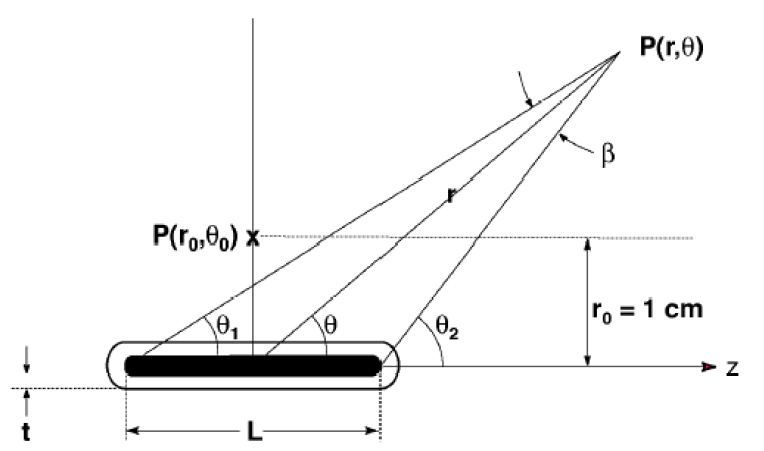
\includegraphics[width=0.7\textwidth]{pictures/geometry}
\caption{Geometry of a line source}
\label{fig:geometry}	
\end{figure}

\end{description}
\newpage

Figure \ref{fig:doseplot} shows the plotted dose function. It is easily seen that the curve has a realy steep slope. Hence it should be discussed for which radii the given function should be evaluated.

\begin{figure}[htbp]

\centering
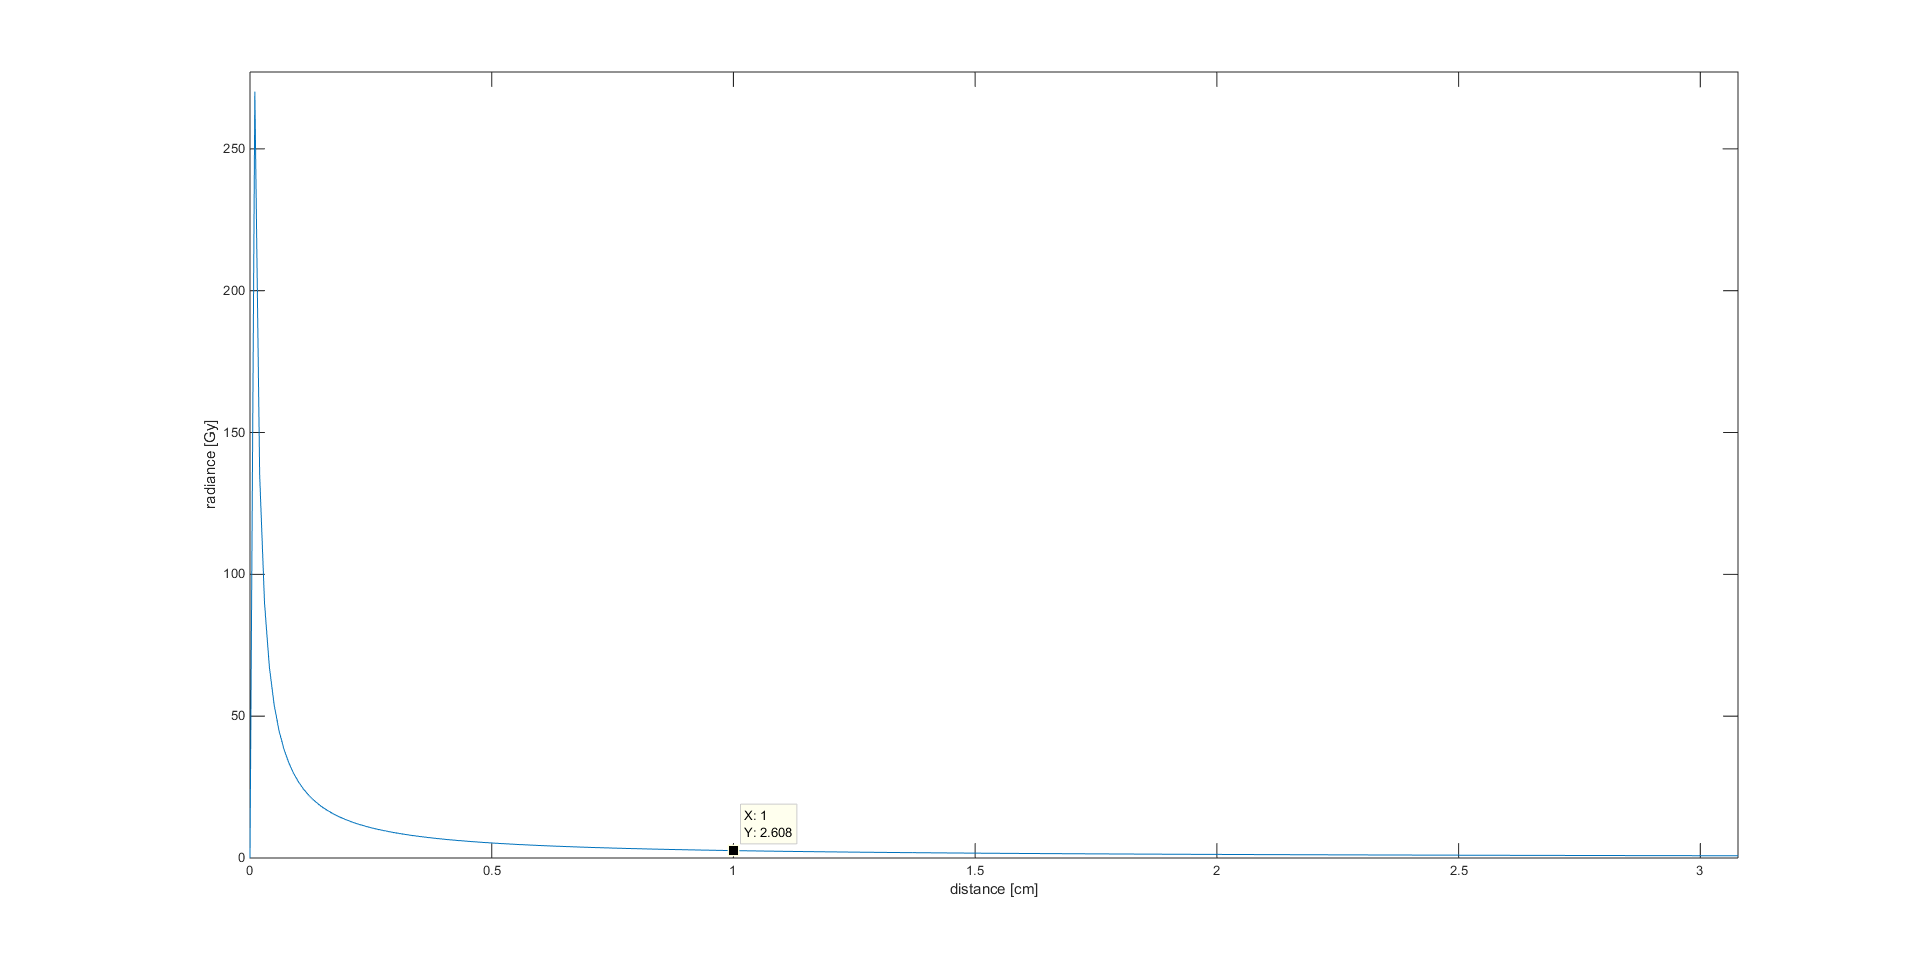
\includegraphics[width=0.9\textwidth]{pictures/dosefunction}
\caption{Dose-Function Plot}
\label{fig:doseplot}
\end{figure}
\section{Genetic Algorithm}
\label{sec:genalg}

Genetic algorithm  or evolutionary algorithm \cite{genpro} describes a search procedure which belongs to the category local search\cite{aima}. Local search algorithms are used when the path to your solution is irrelavant (unlike e.g. breadth first search). The idea of the genetic algorithm is to find the best solution in a solution space by adapting the procedure of genetic reproduction to the problem. \\ 
The algorithm consists mainly of three components:

\begin{description}
\item[Individual] ~\\
\label{indiv}
An individual contains one possible solution for the problem. It could be seen as the interface between the problem and the algorithm.  It is forced to reproduce itself with other individuals so the solution might improve. The key here is to find an efficient encoding for your problem.
\item[Population]~\\
\label{pop}
The sum of all individuals is called population. The population provides the gene pool. Every individual shall reproduce it's gene with another one out of the population. 
\item[Fitness-Function] ~\\
\label{fifu}
The fitnees-function is a heuristic which is used to evaluate the fitness value of an individual. The fitness value indicates how good the solution is, which the individual contains. Further the fitness value is used to select the best individuals for reproduction.
\end{description} 

The genetic algorithm is an iterative algorithm. Each iteration consists of four steps, which are described in the following:

\begin{description}
\item[1. Elitism]~\\
In the elitism step a specific number of the best individuals are taken into the next iteration without further reproduction or other actions. 
\item[2. Selection]~\\
During the selection phase each individual gets selected with a probabilty, that is proportional to it's fitnessvalue.
$P_{selection_{i}}= \tfrac{fitness_{i}}{\sum_{j}^I fitness_{j}}$ Where $I$ is the Population size and $i$ the specific index for a individual.
\item[3. Crossover]~\\
In the crossover step the previously selected individuals are taken pairwise to exchange their solution by using the one point crossover. One point crossover cuts the gene in two parts at a randomly chosen point and exchanges one half of each's gene.



\item[4. Mutation]~\\
In the end each individual changes randomly some parts of it's solution by a given probability.
\end{description}

\subsection{Implementation}
\label{subsec:impl}

The individual is ipmlemented as a $n^{th}$ dimensional vector of the dwell times, where $n$ denotes the number of seeds. Equation \eqref{eq:individual} shows one individual for $n  $ Seeds.
 \begin{equation}
 \label{eq:individual}
 Individual \ \ i := \begin{pmatrix}
 t_{0} \\ \vdots \\ t_{n-1} 	
\end{pmatrix}   
\end{equation} 
 
 The population is, like in \ref{pop} said, the accumulation of all individuals. $k$ denotes the number of individuals.
\begin{equation}
 \label{eq:population}
 Population \ \ p := \begin{pmatrix}
 i_{0} \\ \vdots \\ i_{k-1} 	
\end{pmatrix}   
 \end{equation}
 
 The Fitness-Function calculates the squared differnce between the goaldose and the current dose within the whole body.
 \begin{equation}
 f(individual) = \sum_{body}(GD-CD)^2
 \end{equation}
 For further adjustment and prioritisation the fitness-function is extended by an weighting factor, which holds a specifig weight for any bodytype (tumor, liver, spine,...).
 \begin{equation}
 \label{eq:fifu}
 f(individual) = \sum_{body}w_{bodytype}(GD-CD)^2
 \end{equation}

\subsubsection{Optimisation}
\label{subsubsec:optimisation}
The fitness-function as described in equation \eqref{eq:fifu} is shown in algorithm \ref{alg:fifu}. It is easily seen that it iterates over every voxel in the body. This results in a very high computational complexity and high runtime. To improve the performance of the algorithm three different optimisation approaches are introduced. \\

\begin{algorithm}[H]
\label{alg:fifu}
 $temp=0$\;
 \For{x=0; x $\textless$ body.xDim; x++}{
 	\For{y=0; y $\textless$ body.yDim; y++}{
 		\For{z=0; z $\textless$ body.zDim; z++}{
 			\For{j=0; j $\textless$ numberOfSeeds; j++} {
				 	$temp\ \ = temp+  w_{bodytype}(GD-CD)^2$\;		
 			}
  		}
  	}
  }
 $fitnessvalue = \sqrt{temp}$\;
 \Return{fitnessvalue}\;
 \caption{Calculation of the fitnessvalue}
 
 \end{algorithm}


\paragraph{Scaling}
\label{para:scaling}
~\\
This strategy evaluates not every single voxel in the body. Only every $n^{th}$ voxel is evaluated. Algortithm \ref{alg:scalefif} shows how this is implemented. \\

\paragraph{Treatment Range}
\label{para:treatment range}
~\\
Like the dosefunction chapter has shown, the distribution of the radiation decreases exponential with the distance. This effect could be used to reduce the number of voxel, that has to be evaluated, because the influence of voxels that are relatively far away is negligibly small. Algorithm \ref{alg:scalefif} shows how that information is used. The Region of Interest (roi) denotes the treatment range. \\



\begin{algorithm}[H]
\label{alg:scalefif}

 \For{y=y-roi.min; y $\textless$ y-rio.max; y$\leftarrow$y+Scalefactor}{
 		\For{z=z-roi.min; z $\textless$ z-rio.max; z$\leftarrow$z+Scalefactor}{
 			\For{j=0; j $\textless$ numberOfSeeds; j++} {
				 	$temp\ \ = temp+  w_{bodytype}(GD-CD)^2$\;		
 			}
  		}
  	}
\caption{Optimised Fitness-Function}
\end{algorithm} 






\paragraph{Multithreading}
\label{para:multithreading}
~\\ 
The multithreading approach seperates the 
three-dimensional
body into two-dimensional planes. Each plane is then
processed in an own thread. Algorithm \ref{alg:multithread} shows that approach.\\

 \begin{algorithm}[H]
 \label{alg:multithread}
 \SetKwFunction{cb}{CalculateBounds}
 \SetKwFunction{thread}{ThreadedFitnessFunction}

 \emph{x-roi,y-roi,z-roi $\leftarrow$} \cb{body}  \;
 \For{x-roi}{
 	\thread{x,y-roi,z-roi}
 }
 \caption{Multithreaded Fitness-Function}
 \end{algorithm} 

\subsubsection{Stop Criterion}
\label{subsubsec: stopcrit}
One of the challenges for the genetic algorithm is to decide when and how the algorithm should terminate. It is difficult to detmine how close the current iteration is to the optimal solution. The approach used in this implementation calculates the difference between the current fitness-value and the fitness-value of the previous iteration. If the absolute value of this differnece is less or equal to a small boundary value a counter is incremented. If this counter is incremented five times in a row, the algorithm terminates. \\ 
This procedure shall ensure that small fluctuations, that can accure due to the mutations within the individuals, will have no effect on the termination. \\


\begin{algorithm}[H]
\SetKwFunction{iter}{GeneticAlgIteration}
$individualOld,currentIndividual \leftarrow 0$\;
$stop \leftarrow false$\;
$counter \leftarrow 0$\;
\While{! stop} {
 \tcc{Returns the best fitness value from the current iteration}
 	
	$currentIndividual \leftarrow $\iter{}\;
	
	\If{$\left|individualOld-currentIndividual \right| \ \ \textless \ \ 1$} {
		\emph{counter++}
	} 
	\If{$counter \geq 5$} {
		$done \leftarrow true$
	}  
	$individualOld \leftarrow currentIndividual $
	
	
	
	
	}
	 

\caption{Stop-Criterion}
\end{algorithm}  

\newpage
\subsubsection{Parameters}
The implemented algorithm has a set of parameters, which is used to adjust it's outcome. The usage and the influence of those values are discussed in the following.

\paragraph{Weights}~\\
The fitness-function as described in \ref{fifu} uses individual weighting factors for each body type.  But every tissue type can be weighted with an individual coefficent. 

\paragraph{Probabilities} ~\\ 
There are two important probabilites within the algorithm. The first one is the crossover rate. It describes how likely it is for two individuals to reproduce. The second one is the mutation rate. It describes, analogous to the crossover rate, the probability for an individual to perform a mutation. 

\paragraph{Scaling and Accuracy}~\\
The fitness-function for the given optimisation problem has very high computational complexity. Hence two scaling parameters are introduced to achieve shorter runtimes. The challenge here is to find a compromise between good accuracy for the optimisation and practicable runtimes.\\ The first parameter is the treatment range. It chooses the range around the PTV which shall be evaluated by the algorithm. The second parameter is a simple scaling value which defines that just every  $n^{th}$ voxel is evaluated. Within the treatment range of course.



\subsubsection{Results}


\paragraph{Weights}
It seems hard to examine a specific sets of weights, that is applicable to any type of patients. The experiment has shown, that a higher weighted treatment has a much higher runtime and the convergency decreases.  Figure \ref{fig:weights} shows the difference between the goal dose and the actual dose for different weighted distributions.
\begin{figure}[hbtp]
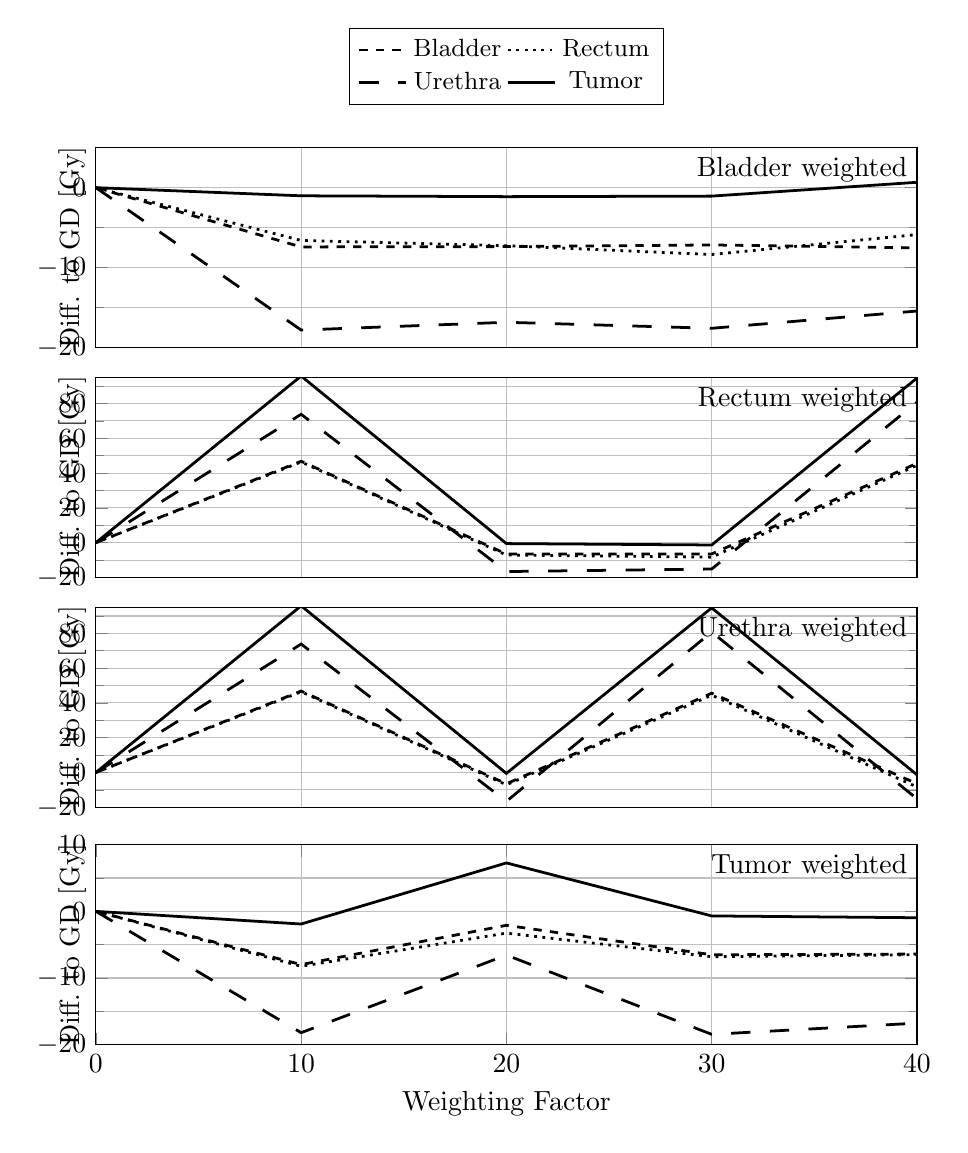
\begin{tikzpicture}
  \begin{axis}[
  	name=one,
  	width=0.86 \columnwidth,
  	height=1.0in, 
  	scale only axis,
  	xmajorticks=false,
  	xtick={0,10,20,30,40},
  	ytick={-20,-10,...,10},
  	minor ytick={-20,-15,...,10},
  	legend style={anchor=north,at={(0.5,1.6)},font=\small},
  	legend columns=2,
    xmin=0,
    xmax=40,
  	ymax = 5,
  	ymin = -20,
    grid=both,
    y label style={at={(axis description cs:0,.5)},anchor=south},
    ylabel = {Diff. to GD [Gy]}
    ]
	\addplot [color=black,dashed,line width=1.0pt]
	table[row sep=crcr]{0 0\\
						10 -7.4061373\\
						20 -7.3660937\\
						30 -7.16107\\
						40 -7.5223036\\	};
	\addlegendentry{Bladder};	
	

	
	\addplot [color=black,dotted,line width=1.0pt]
	table[row sep=crcr]{0 0\\
						10 -6.6003648\\
						20 -7.250544\\
						30 -8.3557603\\
						40 -5.8634733\\ };
	\addlegendentry{Rectum};   
   
    
	
	\addplot [color=black,dash pattern=on 7pt off 7pt,line width=1.0pt]
	table[row sep=crcr]{0 0\\
						10 -17.7968793\\
						20 -16.8252388\\
						30 -17.5772547\\
						40 -15.4201025\\ };
	\addlegendentry{Urethra};
	
	\addplot [color=black,solid,line width=1.0pt]
	table[row sep=crcr]{0 0\\
	 					10 -1.0171151\\
	 					20 -1.1222384\\
				 		30 -1.0559538\\
	 					40  0.6725971\\};
	\addlegendentry{Tumor};					
  \node at (rel axis cs:1,1) [anchor=north east] {Bladder weighted};	
  \end{axis}
  
  \begin{axis}[
  	name=two,
  	width=0.86 \columnwidth,
  	height=1.0in, 
  	scale only axis,
  	at=(one.below south),
    anchor=above north,
  	xmajorticks=false,
  	xtick={0,10,20,30,40},
  	ytick={-20,-0,...,100},
  	minor ytick={-10,0,...,100},
    xmin=0,
    xmax=40,
  	ymax = 95,
  	ymin = -20,
    grid=both,
    y label style={at={(axis description cs:0,.5)},anchor=south},
    ylabel = {Diff. to GD [Gy]}
    ]
	\addplot [color=black,dashed,line width=1.0pt]
	table[row sep=crcr]{0 0\\
						10 46.8163804\\
						20 -6.5099569\\
						30 -6.4596163\\
						40 45.5999754\\ };

	%\addlegendentry{Bladder};	
	
	\addplot [color=black,dotted,line width=1.0pt]
	table[row sep=crcr]{0 0\\
						10 46.4315353\\
						20 -7.0846292\\
						30 -8.312817\\
						40 44.4589502\\ };

	%\addlegendentry{Rectum};   
   
    
	
	\addplot [color=black,dash pattern=on 7pt off 7pt,line width=1.0pt]
	table[row sep=crcr]{0 0\\
						10 73.834936\\
						20 -16.600937\\
						30 -15.1440168\\
						40	80.79331\\  };
	%\addlegendentry{Urethra};
	
	\addplot [color=black,solid,line width=1.0pt]
	table[row sep=crcr]{0 0\\
	 					10 95.820661\\
	 					20 -0.5231224\\
	 					30 -1.3135843\\
	 					40	94.652913\\ };
	%\addlegendentry{Tumor};					
  \node at (rel axis cs:1,1) [anchor=north east] {Rectum weighted};	
  \end{axis}
  \begin{axis}[
  	name=three,
  	width=0.86 \columnwidth,
  	height=1.0in, 
  	scale only axis,
  	at=(two.below south),
    anchor=above north,
  	xmajorticks=false,
  	xtick={0,10,20,30,40},
  	ytick={-20,-0,...,100},
  	minor ytick={-10,0,...,100},
  	legend style={anchor=north,at={(0.5,1.3)},font=\small},
  	legend columns=2,
    xmin=0,
    xmax=40,
  	ymax = 95,
  	ymin = -20,
    grid=both,
    y label style={at={(axis description cs:0,.5)},anchor=south},
    ylabel = {Diff. to GD [Gy]}
    ]
	\addplot [color=black,dashed,line width=1.0pt]
	table[row sep=crcr]{0 0\\
						10 46.8163804\\
						20 -6.5099569\\
						30 45.5999754\\
						40 -6.4596163\\ };

	%\addlegendentry{Bladder};	
	
	\addplot [color=black,dotted,line width=1.0pt]
	table[row sep=crcr]{0 0\\
						10 46.4315353\\
						20 -7.0846292\\
						30 44.4589502\\
						40 -8.312817\\ };

	%\addlegendentry{Rectum};   
   
    
	
	\addplot [color=black,dash pattern=on 7pt off 7pt,line width=1.0pt]
	table[row sep=crcr]{0 0\\
						10 73.834936\\
						20 -16.600937\\
						30 80.79331\\
						40 -15.1440168\\ };
	%\addlegendentry{Urethra};
	
	\addplot [color=black,solid,line width=1.0pt]
	table[row sep=crcr]{0 0\\
	 					10 95.820661\\
	 					20 -0.5231224\\
	 					30 94.652913\\
	 					40 -1.3135843\\ };
	%\addlegendentry{Tumor};					
  \node at (rel axis cs:1,1) [anchor=north east] {Urethra weighted};	
  \end{axis}
  \begin{axis}[
  	name=four,
  	width=0.86 \columnwidth,
  	height=1.0in, 
  	scale only axis,
  	at=(three.below south),
    anchor=above north,
  	xmajorticks=true,
  	xtick={0,10,20,30,40},
  	ytick={-20,-10,...,10},
  	minor ytick={-15,-10,...,5},
    xmin=0,
    xmax=40,
  	ymax = 10,
  	ymin = -20,
    grid=both,
    xlabel = {Weighting Factor},
    y label style={at={(axis description cs:0,.5)},anchor=south},
    ylabel = {Diff. to GD [Gy]}
    ]
	\addplot [color=black,dashed,line width=1.0pt]
	table[row sep=crcr]{0 0\\
						10 -7.9814571\\
						20 -2.0920392\\
						30 -6.5044591\\
						40 -6.4056077\\ };

	%\addlegendentry{Bladder};	
	
	\addplot [color=black,dotted,line width=1.0pt]
	table[row sep=crcr]{0 0\\
						10 -8.2390329\\
						20 -3.2641176\\
						30 -6.7960123\\
						40 -6.5058489\\ };

	%\addlegendentry{Rectum};   
   
    
	
	\addplot [color=black,dash pattern=on 7pt off 7pt,line width=1.0pt]
	table[row sep=crcr]{0 0\\
						10 -18.198227\\
						20 -6.5576085\\
						30 -18.4460054\\
						40 -16.7663932\\ };
	%\addlegendentry{Urethra};
	
	\addplot [color=black,solid,line width=1.0pt]
	table[row sep=crcr]{0 0\\
	 					10 -1.8981359\\
	 					20 7.2659238\\
	 					30 -0.6839885\\
	 					40 -0.955956\\ };
	%\addlegendentry{Tumor};					
  \node at (rel axis cs:1,1) [anchor=north east] {Tumor weighted};	
  \end{axis}
  
\end{tikzpicture}
\caption{Difference between the goal dose and the average dose}
\label{fig:weights}
\end{figure}

\newpage
\paragraph{Probabilities} 
The results have shown, that a high mutation rate leads to a very low tumor coverage. Furthermore the algorithm often doesn't converges, because the changes of the individuals accure too often. A stable state becomes less likely. \\ For the crossover rate the results showed, that the value should be between 0.7 and 0.9.
% Please add the following required packages to your document preamble:
% \usepackage{multirow}
\begin{table}[h]
\label{table:probabilities}
\begin{tabular}{c|ccccc}
\textbf{MR}          & \textbf{CR :}     & 0.3   & 0.5   & 0.7   & 0.9   \\ \hline
\multirow{2}{*}{0.3} & \textbf{CI}       & 1,092 & 1,019 & 1,683 & 1,101 \\
                     & \textbf{Coverage} & 0,778 & 0,387 & 1,000 & 0,770 \\ \hline
\multirow{2}{*}{0.5} & \textbf{CI}       & 1,028 & 1,032 & 1,022 & 1,079 \\
                     & \textbf{Coverage} & 0,360 & 0,410 & 0,395 & 0,403 \\ \hline
\multirow{2}{*}{0.7} & \textbf{CI}       & 1,007 & 1,046 & 1,012 & 1,035 \\
                     & \textbf{Coverage} & 0,281 & 0,316 & 0,011 & 0,341 \\ \hline
\multirow{2}{*}{0.9} & \textbf{CI}       & 1,034 & 1,000 & 1,109 & 1,043 \\
                     & \textbf{Coverage} & 0,256 & 0,001 & 0,736 & 0,273 \\
\end{tabular}
\caption{Mutation rate and coverage for different mutation-  \& crossover rates}

\end{table}
\subsubsection{Scaling and Accuracy}
The dose distribution of a radioactive seed shows that the dose at a radius of 10 cm is negligible small. So any treatment range higher than 10 cm wouldn't lead to better results. 


\section{Linear Programming}
In Linear Programming an objective function and constraints are used to compute the optimal solution to a minimization or maximization problem, as described in [?]. The problem consists of a certain number of variables and a feasible region, which is defined by the contraints. 
Equation \eqref{eq:LPMatrix} shows the standard form of a linear problem. The objective function, modeled with \textit{c},  is to be minimized, while the constraints, modeled with \textit{A} and \textit{b}, are satisfied. The used algorithm yields a vector x for the optimal solution.

 \begin{equation}
 \label{eq:LPMatrix}
 \begin{aligned}
 A \in \mathbb{R}^{m,n}, \ \ \ b \in \mathbb{R}^m, \ \ \ c \in \mathbb{R}^n, \ \ \ x \in \mathbb{R}^n \\
 objective function \ \ \ c^Tx = Min! \\
 min\{c^Tx|Ax \leq b, x \geq 0\}
\end{aligned}
 \end{equation}
 
 
 
 \subsection{Implementation}
 
For our problem we used CPLEX, an implementation of the simplex algorithm by IBM[?]. In simplex the feasible region is considered a polyhedron. The optimal solution must be in one of the vertices of the polyhedron. Simplex finds a start vertex and approaches the optimal solution by going on an edge from vertex to vertex, until there is no better solution.
The constraints allow us a good modelling of the tumor, since we are able to define a constraint with certain limits for each body type.

\paragraph{Basic Funtionality}
The basic functionality is depicted in algorithm \ref{alg:cplex}. This implementation checks every voxel of the body, if it is a tumor voxel or not. In case of a tumor voxel the influence of the radiation of every seed will be summed up, building a greater-equal constraint. For body voxel the influence of the radiation builds a term for the objective function. 
\begin{algorithm}
\label{alg:cplex}
 \For{x=0; x $\textless$ body.xDim; x++}{
 	\For{y=0; y $\textless$ body.yDim; y++}{
 		\For{z=0; z $\textless$ body.zDim; z++}{
			\If{$body[x][y][z].getBodyType() == tumorType$} {
				\For{i=0; i $\textless$ numberOfSeeds; i++}{
					$dosepart[i] \gets cplex.prod(dose(x,y,z,i),time[i])$	
				}
				$cplex.addGe(cplex.sum(dosepart),goalDosis(x,y,z));$
				}
			\Else{\For{i=0; i $\textless$ numberOfSeeds; i++}{
					$objective.addTerm(dose(x,y,z,i),time[i]);$	
				}
				
				
				}
 			
  		}
  	}
  }
  $cplex.addMinimize(objective);$\\
  $cplex.solve();$
 \caption{basic functionality}
 \end{algorithm}



\subsection{Stepwise Approach}




\bibliographystyle{plain}
\bibliography{lit}
\end{document}
